\begin{figure}[p]
\centering
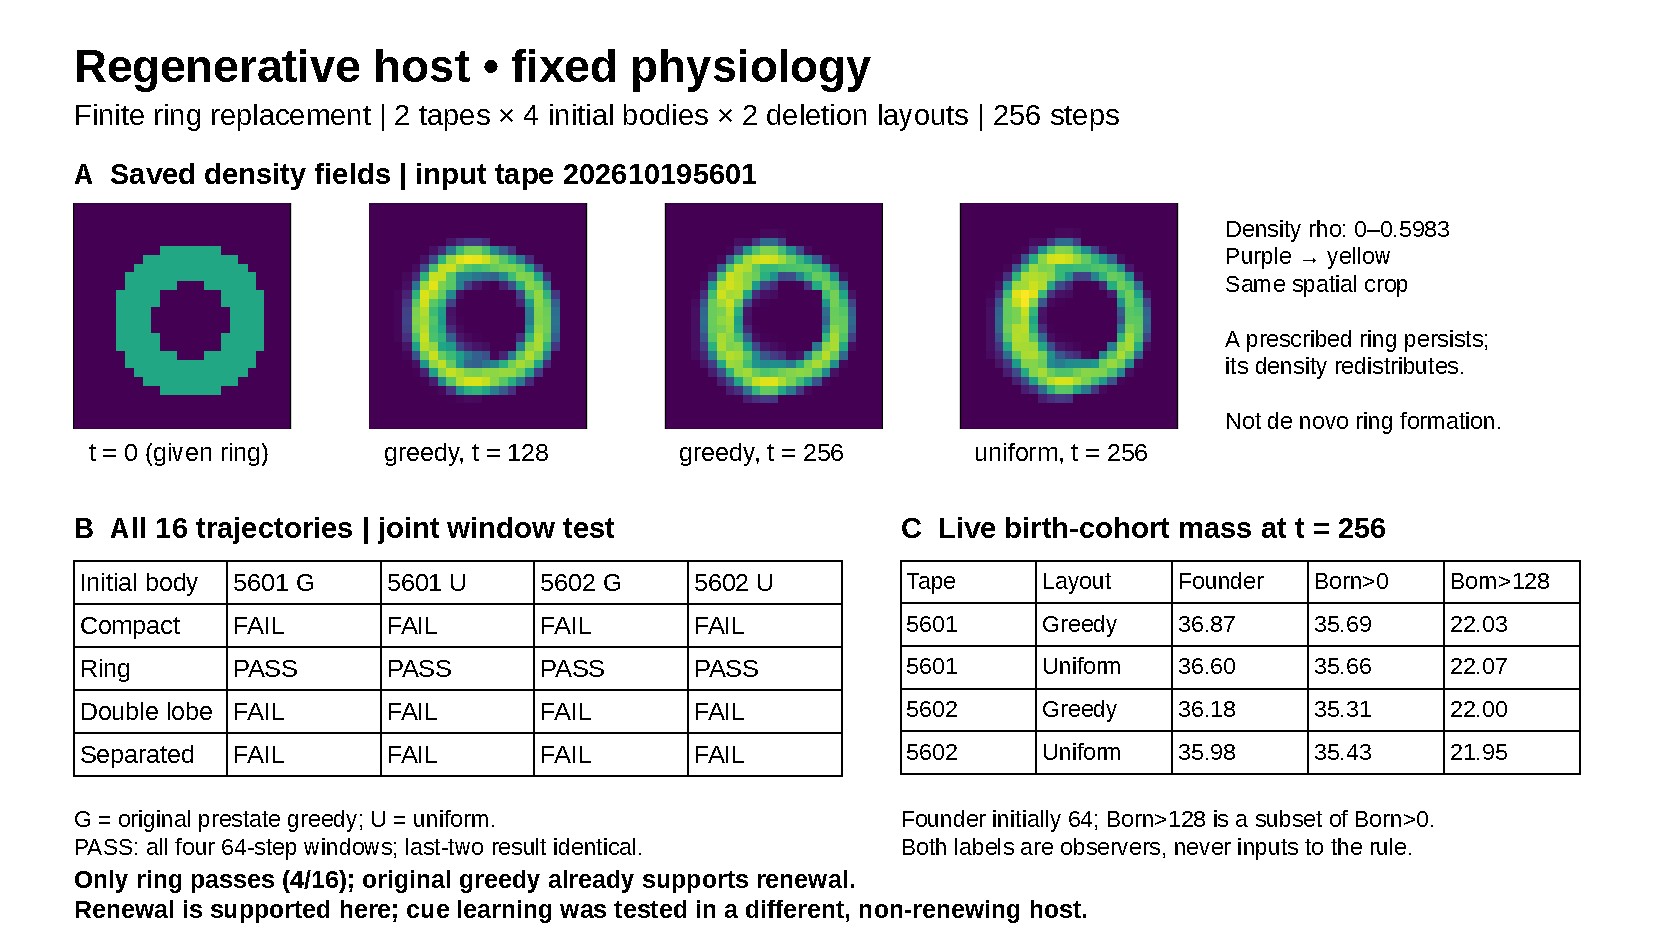
\includegraphics[width=\linewidth,height=.76\textheight,keepaspectratio]{work/longform_v047/figures/finite_replacement_v0474/finite_replacement.pdf}
\caption{\textbf{Finite replacement in a regenerative host under fixed physiology.}
\textbf{A}, Saved density fields for input tape 5601 show the prescribed initial ring and its continuation under original-greedy and uniform deletion layouts, with a common density scale and spatial crop. \textbf{B}, Two tapes, four initial shapes and two layouts give sixteen life-zero trajectories. Both ring seeds under both layouts pass all four fixed 64-step maintenance windows; the other twelve paths fail the final two-window criterion. \textbf{C}, Registered material amounts at step 256 distinguish retained founders from tissue born after life zero and after step 128. The latter is a subset of the former newborn category, not an additional disjoint cohort. Founders start at mass 64. The original rule already supports the ring result; uniform deletion coordination is not necessary. Initial rings are prescribed, not generated from compact starts. These regenerative bodies are distinct from the non-renewing cue-learning hosts in Figs.~\ref{fig:lifetime-learning} and \ref{fig:temporal-credit}; the experiments are not successive phases of one life. The finite 256-step result establishes neither a steady state nor learning, and additional deletion-coordination arithmetic is not physically priced.}
\label{fig:finite-replacement}
\end{figure}
